% Provenance (never printed): see sources/outline_sources.md (Year 2: the vanished ocean;
% ophiolites; nappes; high-pressure rocks; foreland basins; reconstructing the history from
% maps, sections and geophysics). Units, ages and architecture after Schmid et al. (2004);
% Monte Cervino sheet notes (ISPRA 2016); Penrose definition as quoted by Coleman (1984);
% Zermatt-Saas ages Rubatto et al. (1998), Halama et al. (2020); Chenaillet Corno et al.
% (2023); Moho picks Michailos et al. (2023, Zenodo, CC BY 4.0); gravity Zahorec et al.
% (2021); Jura Lanza et al. (2022), Schori et al. (2015); shortening Rosenberg et al.
% (2021); Glarus thrust Herwegh et al. (2008); Molasse Krenmayr (1999), Garefalakis and
% Schlunegger (2018), Sinclair (1997); present uplift Champagnac et al. (2009). Figure data
% in figdata/bachelor-2/alps.py; exercise and problem values in the Book 4 scratch
% calculator calc/ch13.py.
\chapter{Anatomie van een gebergtegordel: de Alpen}\label{ch:b2:alpine-orogen}

De top van de Matterhorn bestaat uit gneis en gabbro die ooit tot de rand van
Apulië behoorden, het continent aan de kant van Afrika van een verdwenen oceaan. De hellingen eronder
zijn de bodem van die oceaan, serpentiniet, gabbro en kussenbasalt die eclogiet werden, en
daaronder, in de naburige Monte Rosa, ligt de rand van Europa. Wie door de
stapel klimt, gaat van het ene continent, door een oceaan, naar het andere. Dit hoofdstuk leest de Alpen als zo'n stapel: waar de stukken vandaan kwamen, hoe ze
werden gestapeld, hoeveel grond het stapelen opslokte, en wat de geofysica eronder ziet.
% ledger: ispra16:cervino, schmid04:apulia, schmid04:alpine-tethys

\begin{recall}
\textbf{Uit Boek~2}: continentale botsing, de sutuur, de verkorting van een
laag (de fractie van haar lengte die verloren gaat), opschuivingen en overschuivingen. \textbf{Uit
Boek~3}: geologische kaarten en doorsneden; afschuivingen, opschuivingen en overschuivingen, plooien en
vergentie; passieve randen; de oceanische korst, kussenlava en het complex van parallelle \omterm{def:b2:magma-emplacement:bodies}{gangen};
actieve randen en het accretieprisma; isostasie, de wortel van Airy en de Bouguer-anomalie;
het \omterm{def:b2:alpine-orogen:foreland}{voorlandbekken}, genoemd onder de sedimentaire bekkens. \textbf{Uit
\cref{ch:b2:metamorphic-facies}}: de blauwschist- en de eclogietfacies. \textbf{Uit
\cref{ch:b2:pt-paths}}: \omterm{def:b2:pt-paths:ptt}{P--T--t-paden}, exhumatiesnelheden en
\omterm{def:b2:pt-paths:uhp}{ultrahogedrukmetamorfose}.
\end{recall}

\begin{definition}[Orogeen]\label{def:b2:alpine-orogen:orogen}
Een \emph{orogeen}\index{orogeen} is een gordel van de lithosfeer die door de
convergentie van twee platen is verkort en verdikt, samen met de gesteenten die erin vervormd en gemetamorfoseerd zijn; de
bergketen is zijn uiting aan het oppervlak, de verdikte korst eronder is zijn wortel.
\end{definition}

\section{Een verdwenen oceaan}\label{sec:b2:alpine-orogen:tethys}

De Alpen leggen de sluiting van oceanen vast terwijl de Afrikaanse en de Europese plaat convergeerden.
De belangrijkste is de \emph{Alpiene Tethys}, bestaande uit twee takken. Haar zuidelijke tak, de
Piemont--Ligurische oceaan, begon in het Midden-Jura uiteen te drijven, toen de Centrale Atlantische
Oceaan openging: de Alpiene Tethys hoort kinematisch bij het opengaan van de Atlantische Oceaan, anders dan de
Tethysoceanen verder naar het oosten. Radiolarieten, kiezelige slikken van de diepzee die gesteente werden,
en aptychuskalksteen volgden op het begin van de spreiding, en ze identificeren nog steeds haar
resten. Een smalle noordelijke tak, de Valais-oceaan, ging waarschijnlijk open in het vroegste
Krijt. Tussen beide lag een reep continent, het Briançonnais-lint, dat naar het oosten
dunner wordt en in de Oostelijke Alpen ontbreekt.
% ledger: schmid04:alpine-tethys

In het noorden werd de oceaan begrensd door de passieve rand van Europa, het onderwerp van het hoofdstuk over
riften en randen in Boek~3. In het zuiden lag \emph{Apulië}: alle continentale
grond ten zuiden van de Alpiene Tethys en ten noorden van de jongere Neotethys, inclusief het voorland
dat nu ten zuiden van de Alpen ligt. De top van de Matterhorn is er een stuk van.
% ledger: schmid04:apulia
De kaart hieronder situeert de gordel en de plaatsen van dit hoofdstuk.

\begin{omfigure}
\centering
% ledger: data:b4-etopo-alps, schmid04:windows, schmid04:foreland, ispra16:cervino
\begin{tikzpicture}
\begin{axis}[width=0.96\linewidth, height=0.74\linewidth, xmin=5, xmax=14, ymin=43.5,
  ymax=48.5, xlabel={lengtegraad (\unit{\degree} OL)}, ylabel={breedtegraad (\unit{\degree} NB)},
  tick label style={font=\scriptsize}, label style={font=\small}, clip=true,
  xtick={5,6,...,14}, ytick={44,45,...,48}]
\addplot[omThm!35, line width=0.3pt] table[x=lon, y=lat] {figdata/out/bachelor-2-alps-c1000.dat};
\addplot[omThm!90!black, line width=0.45pt] table[x=lon, y=lat] {figdata/out/bachelor-2-alps-c2000.dat};
\addplot[blue!60!black, line width=0.5pt] table[x=lon, y=lat] {figdata/out/bachelor-2-alps-c0.dat};
\draw[red!70!black, line width=1pt] (axis cs:8,45.3) -- (axis cs:8,48.0);
\node[font=\scriptsize\bfseries, red!70!black, anchor=north west] at (axis cs:8.02,45.32) {A};
\node[font=\scriptsize\bfseries, red!70!black, anchor=south west] at (axis cs:8.02,47.98) {B};
\fill (axis cs:6.865,45.833) circle (1.3pt) node[font=\scriptsize, fill=white, fill opacity=0.85, text opacity=1, inner sep=1pt, anchor=north east] {Mont Blanc};
\fill (axis cs:7.659,45.976) circle (1.3pt) node[font=\scriptsize, fill=white, fill opacity=0.85, text opacity=1, inner sep=1pt, anchor=south east] {Matterhorn};
\node[font=\scriptsize\itshape, rotate=40] at (axis cs:6.35,46.85) {Jura};
\node[font=\scriptsize\itshape] at (axis cs:9.35,47.65) {Molassebekken};
\node[font=\scriptsize\itshape] at (axis cs:10.0,45.05) {Povlakte};
\node[font=\scriptsize\itshape, align=center, fill=white, fill opacity=0.8, text opacity=1, inner sep=1pt] at (axis cs:10.3,46.95) {Engadin-\\venster};
\node[font=\scriptsize\itshape, align=center, fill=white, fill opacity=0.8, text opacity=1, inner sep=1pt] at (axis cs:12.6,47.25) {Tauern-\\venster};
\node[font=\scriptsize\itshape] at (axis cs:8.6,43.85) {Ligurische Zee};
\end{axis}
\end{tikzpicture}
\par\smallskip{\small De Alpen volgens het reliëfmodel ETOPO1, met een knoop om de \qty{0.05}{\degree}:
hoogtelijnen op \qty{1000}{m} (licht) en \qty{2000}{m} (donker) en de kustlijn. De
hoogste knoop van dit rooster ligt op \qty{3914}{m}, bij de Mont Blanc; de toppen zijn hoger,
omdat een roosterknoop een cel bemonstert, geen piek. De lijn A--B langs \qty{8}{\degree} OL is
het profiel dat in de laatste paragraaf van het hoofdstuk wordt getekend. Namen met de hand geplaatst op hun
geschatte posities.}
\end{omfigure}

Hoe kan men een oceaan kennen die verdwenen is? Door stukken van zijn bodem die aan de
subductie ontsnapten en in de gebergtegordel werden ingeklemd.

\begin{definition}[Ofioliet; Penrose-ofiolietreeks]\label{def:b2:alpine-orogen:ophiolite}
Een \emph{ofioliet}\index{ofioliet} is een kenmerkende associatie van mafische tot ultramafische
gesteenten, een stuk oceanische lithosfeer dat nu op het land voorkomt. De
\emph{Penrose-ofiolietreeks}\index{Penrose-ofiolietreeks} is de volledige associatie die in 1972 door een
conferentie van geologen werd gedefinieerd; van onder naar boven:
\begin{enumerate}
\item een ultramafisch complex van \omterm{def:b2:mantle-melting:peridotites}{harzburgiet}, \omterm{def:b2:mantle-melting:peridotites}{lherzoliet} en \omterm{def:b2:mantle-melting:peridotites}{duniet}, meestal met een
vervormingsmaaksel dat in vaste toestand is verworven;
\item een gabbrocomplex, gewoonlijk met cumulustexturen;
\item een mafisch complex van parallelle \omterm{def:b2:magma-emplacement:bodies}{gangen};
\item een mafisch vulkanisch complex, vaak met kussens.
\end{enumerate}
\end{definition}
% ledger: coleman84:penrose

De definitie van Penrose was een consensus, vanaf het begin bekritiseerd, en nog steeds algemeen
aanvaard. Haar reeks is de gelaagdheid van de oceanische korst en de bovenmantel uit
Boek~3: kussenlava's boven parallelle \omterm{def:b2:magma-emplacement:bodies}{gangen} boven gabbro boven de mantel. \omterm{def:b2:alpine-orogen:ophiolite}{Ofiolieten} zijn echter geen
gemiddelde oceaanbodem. De meeste abyssale korst, de korst van de wijde oceanen, wordt door
subductie verbruikt; Coleman betoogde dat de \omterm{def:b2:alpine-orogen:ophiolite}{ofiolieten} van de Alpiene en Cordillerische gordels
vooral ontstonden in de spreidingscentra van kleine oceaanbekkens of tussen eilandbogen, en dat de
Tethysofiolieten ontstonden waar continentale korst langs passieve randen dunner werd tot er een kleine
oceaan openging.
% ledger: coleman84:penrose, coleman84:settings

De Alpiene \omterm{def:b2:alpine-orogen:ophiolite}{ofiolieten} passen in dat beeld. De eenheden die van de Piemont--Ligurische oceaan afkomstig zijn,
zijn relicten van oceanische lithosfeer en van mantel die van onder het
verdunde continent was opgehaald, de subcontinentale mantel, en op de zeebodem werd blootgelegd. Bij de
Chenaillet, in de Westelijke Alpen, toont de best bewaarde van hen blootgelegde
mantel, gabbro's en een beroemde opeenvolging van kussenbasalten, zonder sedimentair dek.
De foto hieronder toont ze.
% ledger: schmid04:units, corno23:chenaillet

\begin{omfigure}
\centering
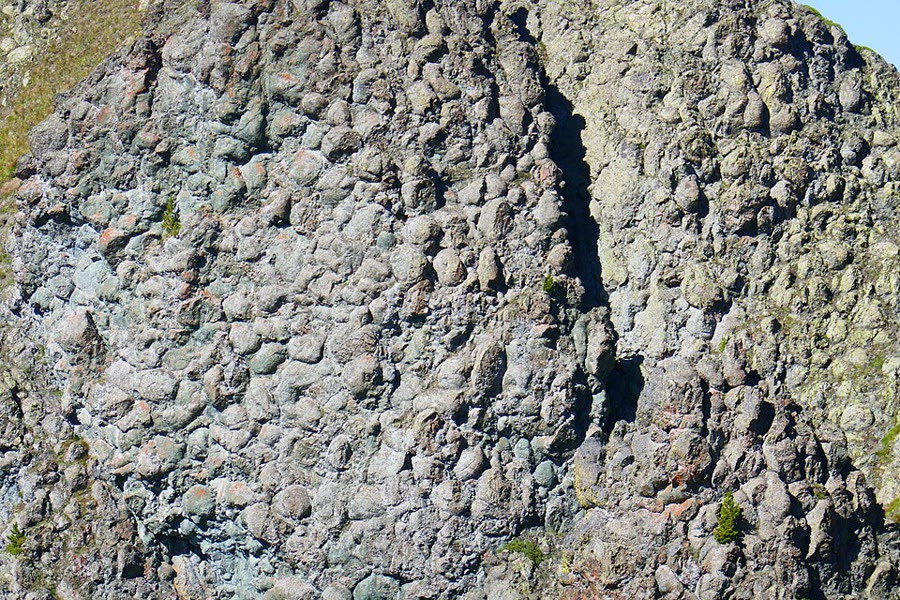
\includegraphics[width=0.66\linewidth]{images/book4/b2-13-pillow-lava.jpg}
\par\smallskip{\small Kussenlava's van de \omterm{def:b2:alpine-orogen:ophiolite}{ofioliet} van de Chenaillet, Westelijke Alpen: elk afgerond
kussen is een lob basalt die uitvloeide en afschrikte op de bodem van de Piemont--Ligurische
oceaan. Foto Lionel Duchoiselle, CC BY-SA 3.0.}
\end{omfigure}

De oceaanbodem kan worden gedateerd waar zijn gabbro's kristalliseerden. Zirkonen uit twee metagabbro's van
de \omterm{def:b2:alpine-orogen:ophiolite}{ofioliet} van Zermatt--Saas, onder de Matterhorn, geven $164.0 \pm \qty{2.7}{Ma}$ en $163.5
\pm \qty{1.8}{Ma}$, en de mangaanrijke sedimenten die op de basalten zijn afgezet, zijn hoogstens $161
\pm \qty{11}{Ma}$ oud: de bodem van de Piemont--Ligurische oceaan werd in het Jura gevormd,
ongeveer \qty{164}{Myr} geleden.
% ledger: rubatto98:zsf

\section{Een oceaan subduceren, en dan een continent}\label{sec:b2:alpine-orogen:subduction}

Een oceaan sluit door subductie. Een deel van zijn bodem belandt echter bovenop een continent
in plaats van eronder, en sommige continenten volgen de oceaan naar beneden.

\begin{definition}[Obductie; continentale subductie]\label{def:b2:alpine-orogen:obduction}
\emph{Obductie}\index{obductie} is het plaatsen van een plaat oceanische lithosfeer op
een continentale rand, waarbij de \omterm{def:b2:alpine-orogen:ophiolite}{ofioliet} over het continent schuift. \emph{Continentale
subductie}\index{continentale subductie} is het afdalen van continentale lithosfeer, getrokken
door de eraan vastzittende oceanische plaat, in een subductiezone nadat de oceaan ervoor
is verbruikt.
\end{definition}

\omterm{def:b2:alpine-orogen:obduction}{Obductie} vond plaats in de Dinariden, ten zuidoosten van de Alpen: \omterm{def:b2:alpine-orogen:ophiolite}{ofiolieten} van de Jurassische
Vardaroceaan, zelf van Midden-Jurassische ouderdom, werden in het Laat-Jura op een
accretiewig en op de rand van Apulië geschoven. Lang werd gedacht dat ze ook de
\omterm{def:b2:alpine-orogen:ophiolite}{ofioliet} van de Chenaillet had geplaatst, omdat zijn gesteenten slechts een zeer laaggradige Alpiene
\omterm{def:b2:metamorphic-facies:metamorphism}{metamorfose} tonen. Een recente studie vond relicten van lawsoniet en omfaciet in zijn gabbro en
albitiet, die zijn Alpiene piek op 10 tot \qty{11}{kbar} en 340 tot
\qty{360}{\celsius} brengen: het gewicht van een \omterm{def:b2:alpine-orogen:nappes}{dekbladstapel} van zo'n 35 tot \qty{40}{km} dik. De auteurs
concluderen dat de Chenaillet gesubduceerd werd, niet geobduceerd, een herinnering dat de lezing van
een \omterm{def:b2:alpine-orogen:ophiolite}{ofioliet} evenzeer op zijn metamorfe geschiedenis berust als op zijn gesteenten.
% ledger: schmid04:obduction, corno23:chenaillet

\subsection*{De oceaan gaat omlaag}

In het Krijt werd de zuidelijke, Apulische rand van de Piemont--Ligurische oceaan een
actieve rand: zijn trog vulde zich met schalie en zandsteen, nu de kalkrijke schisten
die Bündnerschiefer of schistes lustrés heten. De Oostelijke Alpen leggen ook een eerdere
botsing vast, de sluiting van een golf van een andere oceaan, de Meliata, tegen Apulië, met een
hogedrukpiek rond \qty{100}{Ma}: de Alpen zijn het product van twee orogenesen, een
Krijt-orogenese en een Tertiaire.
% ledger: schmid04:two-orogenies

De \omterm{def:b2:alpine-orogen:ophiolite}{ofioliet} van Zermatt--Saas daalde af tot de eclogietfacies van
\cref{ch:b2:metamorphic-facies}: zijn eclogieten bereikten 550 tot \qty{600}{\celsius} en 2.5 tot
\qty{3.0}{GPa}, en de piekdruk werd bereikt tussen 48 en \qty{44}{Ma}. Eén schijf ervan,
bij het Lago di Cignana, bevat coësiet en microscopische diamanten in gesteenten die begonnen als basalten
en sedimenten van de oceaanbodem; ze bereikte ongeveer \qty{615}{\celsius} en \qty{2.8}{GPa}, en haar
zirkonen dateren dat diepste punt op $44.1 \pm \qty{0.7}{Ma}$. Oceaanbodem die
\qty{164}{Myr} geleden ontstond, werd op een ouderdom van 120 miljoen jaar gesubduceerd tot diepten van
\qty{90}{km} of meer, en kwam daarna terug.
% ledger: halama20:cignana, rubatto98:zsf

\subsection*{Het continent volgt}

Toen de oceaan verdwenen was, werd de rand van Europa erachteraan gesleept. De coësiethoudende
kwartsieten van het massief van Dora Maira, ontmoet in \cref{ch:b2:pt-paths}, zijn continentale korst
van de Europese kant van de oceaan die meer dan \qty{90}{km} bereikte, ongeveer
\qty{35}{Myr} geleden, en terugkwam met de snelheid van platen. Het dateren van de hogedrukgesteenten
over de hele gordel geeft een volgorde: de Apulische rand zelf (de Sesiazone) in het
Laat-Krijt, de \omterm{def:b2:alpine-orogen:ophiolite}{ofiolieten} van de Piemont--Ligurische oceaan rond \qty{44}{Ma}, de
Europese continentale korst in het Laat-Eoceen. Rubatto en collega's lezen dat als drie subductie-episoden die in de tijd verspringen van
zuidoost naar noordwest, naar Europa toe.
% ledger: chopin84:coesite, rh01:exhumation, rubatto98:zsf, ispra16:cervino

De botsing volgde: de Valais-oceaan, de laatste oceanische strook, sloot tijdens het midden tot
late Eoceen, en vanaf dat moment werd continentale korst op continentale korst gestapeld.
De figuur hieronder vat de opeenvolging samen.
% ledger: schmid04:alpine-tethys

\begin{omfigure}
\centering
\begin{tikzpicture}[x=0.95cm, y=0.78cm, font=\scriptsize]
% (a) rifting and spreading
\begin{scope}[yshift=0cm]
\node[anchor=west, font=\scriptsize\bfseries] at (-0.2,0.75) {(a) Jura: de oceaan gaat open};
\fill[gray!25] (0,0) -- (3.2,0) -- (3.8,-0.6) -- (0,-0.6) -- cycle;
\fill[gray!25] (6.2,0) -- (10,0) -- (10,-0.6) -- (5.6,-0.6) -- cycle;
\fill[omThm!35] (3.2,0) -- (6.2,0) -- (5.6,-0.6) -- (3.8,-0.6) -- cycle;
\fill[blue!8] (0,0) rectangle (10,0.4);
\draw[thick] (4.7,0) -- (4.7,-0.6);
\node at (1.6,-0.3) {Europa};
\node at (8,-0.3) {Apulië};
\node[align=center] at (4.7,0.2) {rug};
\end{scope}
% (b) oceanic subduction
\begin{scope}[yshift=-1.7cm]
\node[anchor=west, font=\scriptsize\bfseries] at (-0.2,0.75) {(b) Krijt tot Eoceen: de oceaan wordt gesubduceerd};
\fill[blue!8] (0,0) rectangle (7,0.4);
\fill[gray!25] (0,0) -- (3.0,0) -- (3.6,-0.6) -- (0,-0.6) -- cycle;
\fill[omThm!35] (3.0,0) -- (6.3,0) -- (6.0,-0.5) -- (5.6,-0.95) -- (3.6,-0.6) -- cycle;
\fill[gray!25] (6.3,0) -- (6.6,0.3) -- (10,0.3) -- (10,-0.6) -- (6.4,-0.6) -- cycle;
\fill[omThm!35] (5.6,-0.95) -- (6.0,-0.5) -- (7.4,-1.3) -- (7.2,-1.55) -- cycle;
\fill[orange!40] (6.0,0) -- (6.3,0) -- (6.6,0.3) -- (6.35,0.3) -- cycle;
\draw[-{Latex[length=2mm]}] (7.0,-1.0) -- (7.6,-1.38);
\node at (1.6,-0.3) {Europa};
\node at (8.4,-0.15) {Apulië};
\node[anchor=west] at (7.5,-1.1) {eclogiet};
\end{scope}
% (c) continental subduction
\begin{scope}[yshift=-3.95cm]
\node[anchor=west, font=\scriptsize\bfseries] at (-0.2,0.75) {(c) Eoceen: de Europese rand volgt};
\fill[gray!25] (0,0) -- (5.6,0) -- (6.2,-0.5) -- (7.4,-1.35) -- (7.1,-1.6) -- (5.6,-0.6) -- (0,-0.6) -- cycle;
\fill[omThm!35] (6.2,0.05) -- (6.6,0.3) -- (6.95,0.3) -- (6.4,-0.2) -- cycle;
\fill[gray!25] (6.6,0.3) -- (10,0.3) -- (10,-0.6) -- (6.9,-0.6) -- (6.4,-0.2) -- (6.95,0.3) -- cycle;
\draw[dashed] (6.6,-0.85) circle (0.22);
\draw (6.82,-0.9) -- (7.6,-1.2);
\node[anchor=west] at (7.6,-1.2) {UHP continentale korst};
\node at (2.4,-0.3) {Europa};
\node at (8.4,-0.15) {Apulië};
\end{scope}
% (d) collision
\begin{scope}[yshift=-6.65cm]
\node[anchor=west, font=\scriptsize\bfseries] at (-0.2,1.4) {(d) Oligoceen tot heden: botsing, dekbladen, voorlandbekkens};
\fill[yellow!35] (0.6,0) -- (3.4,0) -- (3.4,-0.3) -- cycle;
\fill[gray!25] (0,-0.3) -- (3.4,-0.3) -- (4.2,0.5) -- (5.2,0.75) -- (6.2,0.55) -- (7.0,0.2) -- (10,0.2)
  -- (10,-0.7) -- (6.6,-0.7) -- (5.4,-1.5) -- (4.0,-1.5) -- (3.2,-0.9) -- (0,-0.9) -- cycle;
\draw (3.4,-0.3) -- (4.5,-1.0);
\draw (4.2,0.5) -- (5.6,-0.4);
\draw (5.2,0.75) -- (6.1,0.1);
\fill[omThm!35] (5.05,0.6) -- (5.55,0.68) -- (5.85,0.32) -- (5.4,0.25) -- cycle;
\fill[yellow!35] (7.0,0.2) -- (9.6,0.2) -- (7.0,-0.1) -- cycle;
\node at (1.4,-0.6) {Europa};
\node at (8.6,-0.3) {Apulië};
\node[anchor=south] at (1.9,0.02) {molasse};
\node at (4.7,-1.25) {wortel};
\node[anchor=south west] at (6.25,0.6) {dekbladstapel};
\end{scope}
\end{tikzpicture}
\par\smallskip{\small Een schematische geschiedenis van de Alpen, niet op schaal (oceanische lithosfeer rood,
continentale grijs, accretiewig oranje, \omterm{def:b2:alpine-orogen:foreland}{voorlandbekkens} geel).
(a)~De Piemont--Ligurische oceaan gaat open tussen Europa en Apulië. (b)~Zijn bodem wordt onder
Apulië gesubduceerd en tot eclogiet omgezet. (c)~De Europese rand wordt erachteraan omlaaggetrokken en
bij ultrahoge druk gemetamorfoseerd. (d)~Continentale korst wordt tot \omterm{def:b2:alpine-orogen:nappes}{dekbladen} gestapeld boven een
verdikte wortel, met flexurele \omterm{def:b2:alpine-orogen:foreland}{voorlandbekkens} aan beide kanten.}
\end{omfigure}
% ledger: schmid04:alpine-tethys, schmid04:two-orogenies, rubatto98:zsf, schmid04:foreland

\section{Dekbladen, klippen en vensters}\label{sec:b2:alpine-orogen:nappes}

De stukken oceaan en continent werden niet in hun geheel opgestapeld. Ze werden als dunne
schijven afgeschraapt en ver meegevoerd.

\begin{definition}[Dekblad; dekbladstapel]\label{def:b2:alpine-orogen:nappes}
Een \emph{dekblad}\index{dekblad} is een grote gesteenteplaat, vaak enkele kilometers dik en tientallen
kilometers lang, die langs een flauw hellende overschuiving of in de omgekeerde flank van een grote
liggende plooi ver van zijn plaats van oorsprong is meegevoerd; de gesteenten van een dekblad zijn
\emph{allochtoon}\index{allochtoon (gesteente-eenheid)}, die welke ter plaatse bleven
\emph{autochtoon}\index{autochtoon (gesteente-eenheid)}. Een
\emph{dekbladstapel}\index{dekbladstapel} is een stapel dekbladen waarin de structureel hogere dekbladen
meestal van verder binnen in het \omterm{def:b2:alpine-orogen:orogen}{orogeen} komen.
\end{definition}

In de Alpen is de stapelvolgorde de geografie van de verdwenen oceaan op zijn kop gezet,
en de eenheden zijn genoemd naar hun oorsprong (tabel hieronder).

\begin{omfigure}
\centering\small
\begin{tabular}{>{\raggedright\arraybackslash}p{0.24\linewidth}|>{\raggedright\arraybackslash}p{0.66\linewidth}}
eenheid (van boven naar onder) & oorsprong en gesteenten \\ \hline
Austroalpiene \omterm{def:b2:alpine-orogen:nappes}{dekbladen} & rand van Apulië ten noorden van de Periadriatische Lijn: schijven van
sokkel en dek, losgemaakt van hun onderkorst \\
Margna--Sesia-dekbladen (Sesiazone, Dent Blanche) & fragmenten die bij het opengaan van de oceaan van de buitenste
Apulische rand werden afgescheurd \\
Bovenpenninische \omterm{def:b2:alpine-orogen:nappes}{dekbladen} & Piemont--Ligurische oceaan: \omterm{def:b2:alpine-orogen:ophiolite}{ofiolieten}, geëxhumeerde mantel, kalkrijke
schisten \\
Middenpenninische \omterm{def:b2:alpine-orogen:nappes}{dekbladen} & het lintcontinent van het Briançonnais \\
Onderpenninische \omterm{def:b2:alpine-orogen:nappes}{dekbladen} & Valais-oceaan: \omterm{def:b2:alpine-orogen:ophiolite}{ofiolieten} en kalkrijke schisten \\
Subpenninische \omterm{def:b2:alpine-orogen:nappes}{dekbladen} & Europese sokkel, losgemaakt van zijn onderkorst \\
Helvetische \omterm{def:b2:alpine-orogen:nappes}{dekbladen} & kalksteenrijk dek van de nabije Europese rand, losgemaakt van zijn
sokkel \\ \hline
Zuidelijke Alpen & Apulië ten zuiden van de Periadriatische Lijn: een zuidwaarts gerichte \omterm{def:b2:alpine-orogen:ftb}{plooi- en overschuivingsgordel},
grotendeels Mioceen, 10 tot \qty{15}{km} dik
\end{tabular}
\par\smallskip{\small De belangrijkste tektonische eenheden van de Alpen, van de structurele top
naar beneden, met het domein waaruit elk kwam (naar Schmid en collega's).}
\end{omfigure}
% ledger: schmid04:units, schmid04:apulia

De bovenplaat, Apulië, ligt bovenop; daaronder komen, in volgorde, de verre oceaan, het
Briançonnais, de nabije oceaan en de Europese rand, waarbij de laagste eenheden die zijn die
het dichtst bij Europa lagen. Grote plooien die de \omterm{def:b2:alpine-orogen:nappes}{dekbladen} na het stapelen opnieuw plooiden,
verstoren soms de volgorde, en sommige repen, zoals het Briançonnais, wiggen langs de
gordel uit.
% ledger: schmid04:units, schmid04:alpine-tethys

Erosie snijdt daarna de stapel aan, en twee vormen verschijnen op een kaart.

\begin{definition}[Klippe; tektonisch venster]\label{def:b2:alpine-orogen:klippe}
Een \emph{klippe}\index{klippe} (meervoud klippen) is een geïsoleerd restant van een \omterm{def:b2:alpine-orogen:nappes}{dekblad}, dat
op de gesteenten eronder blijft staan wanneer erosie de rest van de plaat heeft verwijderd; het wordt
omringd door zijn basale overschuiving. Een \emph{tektonisch venster}\index{tektonisch venster} is een gat
dat door een \omterm{def:b2:alpine-orogen:nappes}{dekblad} is uitgesleten, waar de gesteenten onder zijn basale overschuiving verschijnen, omringd door het
\omterm{def:b2:alpine-orogen:nappes}{dekblad}.
\end{definition}

\begin{omfigure}
\centering
\begin{tikzpicture}[x=0.68cm, y=0.68cm, font=\scriptsize]
\def\thrust{(0,0) -- (5,0) .. controls (6.5,0) and (7,1.1) .. (8,1.1)
  .. controls (9,1.1) and (9.5,0) .. (11,0) -- (16,0)}
\def\topo{(0,1.7) .. controls (3,1.9) and (5,1.8) .. (6,1.5) .. controls (7,1.0) .. (8,0.6)
  .. controls (9,1.0) .. (10.3,1.5) .. controls (11.3,1.3) .. (12.5,-0.4)
  .. controls (13.3,0.9) .. (14.5,0.95) .. controls (15.5,0.8) .. (16,-0.2)}
\begin{scope}
\clip \topo -- (16,-2.6) -- (0,-2.6) -- cycle;
\fill[gray!20] (0,-2.6) rectangle (16,2.2);
\fill[omThm!30] \thrust -- (16,2.2) -- (0,2.2) -- cycle;
\draw[gray!55, yshift=-0.9*0.68cm] \thrust;
\draw[gray!55, yshift=-1.8*0.68cm] \thrust;
\draw[line width=1.2pt] \thrust;
\end{scope}
\draw \topo;
\node at (2.5,1.0) {dekblad};
\node[anchor=north west] at (0.2,-0.05) {basale overschuiving};
\node at (3.6,-1.35) {autochtoon};
\draw[-{Latex[length=1.6mm]}] (8,2.0) node[anchor=south] {tektonisch venster} -- (8,0.75);
\draw[-{Latex[length=1.6mm]}] (14.5,2.0) node[anchor=south] {klippe} -- (14.5,1.05);
\end{tikzpicture}
\par\smallskip{\small Een \omterm{def:b2:alpine-orogen:nappes}{dekblad} (kleur) op zijn \omterm{def:b2:alpine-orogen:nappes}{autochtoon} (grijs) na erosie, in een
schematische doorsnede: waar zijn basale overschuiving (dikke lijn) opwelft, heeft erosie het
\omterm{def:b2:alpine-orogen:nappes}{dekblad} doorsneden en een \omterm{def:b2:alpine-orogen:klippe}{tektonisch venster} geopend op de gesteenten eronder; vooraan staat een restant van het
\omterm{def:b2:alpine-orogen:nappes}{dekblad} geïsoleerd op de \omterm{def:b2:alpine-orogen:nappes}{autochtoon}, een \omterm{def:b2:alpine-orogen:klippe}{klippe}.}
\end{omfigure}

De Alpen staan vol met beide. De Matterhorn is een \omterm{def:b2:alpine-orogen:klippe}{klippe}: zijn top hoort bij het overschuivingssysteem van de Dent
Blanche, een erosierest van Apulische gesteenten bovenop de hele wig, zijn
gneisen en gabbro's van Permische ouderdom rustend op de \omterm{def:b2:alpine-orogen:ophiolite}{ofiolieten} van het \omterm{def:b2:alpine-orogen:nappes}{dekblad} van Zermatt--Saas
en de Combinzone, die op hun beurt rusten op de \omterm{def:b2:alpine-orogen:nappes}{dekbladen} van de Monte Rosa en de Grote Sint-Bernhard van de
Europese kant (foto hieronder). Aan het noordelijke front van de
Westelijke Alpen vormen \omterm{def:b2:alpine-orogen:nappes}{dekbladen} van het sedimentaire dek, van ver binnen in de gordel, de Préalpes Romandes en de
\omterm{def:b2:alpine-orogen:klippe}{klippen} van Centraal-Zwitserland. In de Oostelijke Alpen openen zich twee vensters door het
Austroalpiene deksel: het Engadinvenster, waar schisten van de Valais-oceaan met blauwschisten
onder de laatste resten van het Briançonnais verschijnen, en het grotere Tauernvenster, waar de
Europese rand en schijven van de Alpiene Tethys onder de Austroalpiene
\omterm{def:b2:alpine-orogen:nappes}{dekbladen} uit komen.
% ledger: ispra16:cervino, schmid04:windows

\begin{omfigure}
\centering
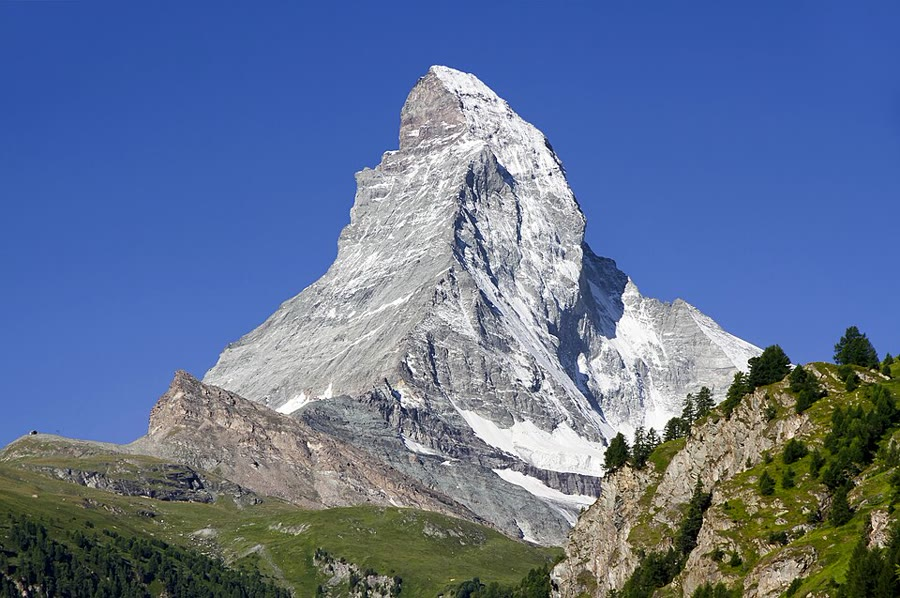
\includegraphics[width=0.7\linewidth]{images/book4/b2-13-matterhorn.jpg}
\par\smallskip{\small De noordoostkant van de Matterhorn (\qty{4478}{m}), gezien vanuit Zermatt:
zijn bovenste piramide is Apulische gneis en gabbro van het overschuivingssysteem van de Dent Blanche, een \omterm{def:b2:alpine-orogen:klippe}{klippe}
op de \omterm{def:b2:alpine-orogen:ophiolite}{ofiolieten} van de Alpiene Tethys. Foto Ximonic (Simo Räsänen), CC BY-SA
4.0.}
\end{omfigure}
% ledger: ispra16:cervino

\subsection*{Onthechtingsvlakken en de twee huiden}

\omterm{def:b2:alpine-orogen:nappes}{Dekbladen} en overschuivingsplaten bewegen over zwakke vlakken.

\begin{definition}[Décollement]\label{def:b2:alpine-orogen:decollement}
Een \emph{décollement}\index{decollement@décollement} is een flauw hellend vlak waarlangs een
gesteenteopeenvolging loskomt van wat eronder ligt en eroverheen glijdt, waarbij beide kanten
onafhankelijk vervormen; het volgt meestal een zwakke laag zoals evaporiet of schalie.
\end{definition}

\begin{definition}[Dunhuidige en dikhuidige tektoniek]\label{def:b2:alpine-orogen:skin}
\emph{Dunhuidige tektoniek}\index{dunhuidige tektoniek} is vervorming van een
sedimentair dek dat langs een basaal \omterm{def:b2:alpine-orogen:decollement}{décollement} van zijn sokkel is losgemaakt: het dek plooit en
overschuift terwijl de sokkel eronder onvervormd blijft. \emph{Dikhuidige
tektoniek}\index{dikhuidige tektoniek} is vervorming waarbij de sokkel betrokken is,
waarbij dek en sokkel samen verkorten langs breuken die tot in de sokkel snijden.
\end{definition}
% ledger: lanza22:jura

\begin{definition}[Plooi- en overschuivingsgordel]\label{def:b2:alpine-orogen:ftb}
Een \emph{plooi- en overschuivingsgordel}\index{plooi- en overschuivingsgordel} is een gordel van plooien en overschuivingen
die het buitenste deel van een \omterm{def:b2:alpine-orogen:orogen}{orogeen} verkort en naar zijn voorland voortschrijdt; overschuivingen
klimmen vanaf het \omterm{def:b2:alpine-orogen:decollement}{décollement} trapsgewijs door de lagen, en plooien groeien erboven.
\end{definition}

De Alpen hebben beide huiden. De Helvetische \omterm{def:b2:alpine-orogen:nappes}{dekbladen} zijn een dunhuidige \omterm{def:b2:alpine-orogen:ftb}{plooi- en overschuivingsgordel}, de
mesozoïsche kalkstenen van de nabije Europese rand, losgemaakt van hun sokkel. Hun basis is
de Glarus-overschuiving, waar Permische rode lagen op cenozoïsche \omterm{def:b2:alpine-orogen:foreland}{flysch} liggen. In het Mioceen werden
daarentegen sokkelblokken van de externe massieven, verkorte en verdikte Europese sokkel (de massieven van de
Aar, de Mont Blanc, Belledonne, Pelvoux en Argentera), met hun
dek opgeschoven: dikhuidige overschuiving.
% ledger: schmid04:units, schmid04:skins, herwegh08:glarus, rosenberg21:massifs

De Jura, de boog van ruggen ten noordwesten van het Zwitserse plateau, is het klassieke voorbeeld van dunne
huid. In het Laat-Mioceen en Plioceen werd zijn mesozoïsche dek geplooid en opgeschoven boven een
\omterm{def:b2:alpine-orogen:decollement}{décollement} in de zwakke evaporieten van het Midden- en Boven-Trias, terwijl de sokkel eronder,
die vanaf de externe massieven onder het Molassebekken doorloopt, er niet bij betrokken was: in
de klassieke lezing kwam de duw van de verre externe massieven. De seismologie heeft sindsdien
een dikhuidig hoofdstuk toegevoegd. De aardbevingen bij Saint-Ursanne in 2000 hadden hun bron
minder dan een kilometer diep en een overschuivingsmechanisme, actieve ondiepe overschuiving in het dek,
terwijl andere studies sokkelbreuken vinden die sinds het jongste Plioceen opnieuw actief zijn. Of
de Jura nog steeds van zijn sokkel is losgemaakt, staat ter discussie.
% ledger: lanza22:jura, schmid04:skins

\begin{inthefield}[Een overschuivingscontact lezen]
Tussen Flims en de Walensee in Oost-Zwitserland loopt de Glarus-overschuiving, een van de
opvallendste grote, flauw hellende overschuivingen van de Alpen. Langs haar liggen Permische rode lagen, het
Verrucano, boven cenozoïsche \omterm{def:b2:alpine-orogen:foreland}{flysch}: veel oudere gesteenten rusten op jongere. Daartussen vormt een
dunne, sterk geschoven band kalksteen het contact: de Lochseiten-kalksteen, waarop de verplaatsing, minstens 30 tot
\qty{40}{km}, zich concentreerde. In de negentiende eeuw las Heim de structuur als twee enorme
omgekeerde plooien die naar elkaar toe gericht waren; Escher von der Linth had er één overschuiving in gelezen, en de lezing als overschuiving won het. Een geoloog die zo'n contact tegenkomt, controleert
drie dingen: of oudere gesteenten op jongere liggen, wat geen gewone gelaagdheid kan;
of de lagen aan weerszijden bij het contact worden afgesneden; en of het contact
zelf een band van geschoven, gerekristalliseerd gesteente is in plaats van een laagvlak.
\end{inthefield}
% ledger: herwegh08:glarus

\section{Voorlandbekkens: flysch en molasse}\label{sec:b2:alpine-orogen:foreland}

Een gebergtegordel belast de plaat waarop hij rust, en de plaat buigt vóór hem omlaag.

\begin{definition}[Voorlandbekken; flysch; molasse]\label{def:b2:alpine-orogen:foreland}
Een \emph{voorlandbekken}\index{voorlandbekken} is een langgerekt sedimentair bekken dat ontstaat
tussen een \omterm{def:b2:alpine-orogen:orogen}{orogeen} en het stabiele continent ervoor, waar de plaat wordt omlaaggebogen door
de last van de overschuivingswig; het is het diepst naast het overschuivingsfront en wordt zelf
geleidelijk overschoven. \emph{Flysch}\index{flysch} is de diepwatervulling van zo'n
bekken, vooral turbidieten van zandsteen en schalie, afgezet zolang het bekken ondergevuld is.
\emph{Molasse}\index{molasse} is zijn latere ondiepmariene en continentale vulling, vooral
conglomeraten en zandstenen uit de eroderende gordel, afgezet zodra de aanvoer het
bekken vult.
\end{definition}
% ledger: sinclair97:trinity, schmid04:foreland, krenmayr99:molasse

Het buigen is elastische flexuur van de lithosfeer, die in een hoofdstuk van
Boek~5 wordt behandeld; hier telt alleen het effect op het bekken. Sinclair beschreef het vroege Alpiene \omterm{def:b2:alpine-orogen:foreland}{voorlandbekken}, van Paleoceen tot Oligoceen,
als een ``ondergevulde drie-eenheid'': kalkstenen aan de continentale kant, hemipelagische modder in het
midden, diepwaterturbidieten tegen het overschuivingsfront. Naarmate de overschuivingen oprukten, schoof het bekken
met hen mee: door Zwitserland kroop zijn continentale kustlijn naar het noordwesten met 8.5
tot \qty{12.9}{mm} per jaar, en het bekken migreerde met een bijna constante vorm over minstens
\qty{210}{km} over de Europese plaat.
% ledger: sinclair97:trinity

Het Noord-Alpiene Molassebekken, dat zich van de Zee-Alpen tot Wenen uitstrekt, begon in het
Laat-Eoceen te dalen. Onder-Oligocene \omterm{def:b2:alpine-orogen:foreland}{flysch}, nu bovenop de Helvetische
\omterm{def:b2:alpine-orogen:nappes}{dekbladen} te vinden, legt een laatste diepwaterstadium vast; van het Laat-Oligoceen tot het Laat-Mioceen
spreidden rivieren continentale grind- en zandlagen uit de jonge bergen. De naam is oud: H.-B. de Saussure
voerde \emph{\omterm{def:b2:alpine-orogen:foreland}{molasse}} in 1779 in. De vulling wordt naar de gordel toe dikker: in de
Oostenrijkse sector tot meer dan \qty{4000}{m} aan het overschuivingsfront, en elders in het bekken
is één enkele Laat-Oligocene reeks rivierconglomeraten zo'n \qty{4}{km} dik. Het zuidelijke deel van
het bekken is overreden: de Oostenrijkse dagzoomgordel, ongeveer \qty{60}{km} breed, is minder
dan een kwart van de vroegere breedte van het bekken. De overreden \omterm{def:b2:alpine-orogen:foreland}{molasse} zelf is in
de overschuivingen gevangen als de Subalpiene \omterm{def:b2:alpine-orogen:foreland}{Molasse}, naar het zuiden hellende schijven conglomeraat langs de
noordrand van de gordel.
% ledger: schmid04:foreland, krenmayr99:molasse, gs18:conglomerates

Ten zuiden van de Alpen ligt de Povlakte op het weinig vervormde Adriatische voorland van de
Zuidelijke Alpen. Haar jongste sedimenten, uit Plioceen en Pleistoceen, bedekken Alpiene
structuren deels discordant en zijn deels vervormd door de laatste overschuivingen van de Zuidelijke Alpen
en van de Apennijnen.
% ledger: schmid04:foreland

\begin{omfigure}
\centering
\begin{tikzpicture}[x=0.5cm, y=0.6cm, font=\scriptsize]
\begin{scope}
\node[anchor=west, font=\scriptsize\bfseries] at (0,2.4) {(a) ondergevuld: flysch};
\fill[blue!8] (0,0) -- (12,0) -- (12,1.4) -- (9.0,1.4) -- (4,0.05) -- (0,0.05) -- cycle;
\fill[gray!25] (0,0) -- (12,-1.1) -- (12,-1.9) -- (0,-0.8) -- cycle;
\fill[omThm!30] (9.0,1.4) -- (12,2.2) -- (12,-1.1) -- (9.5,-0.87) -- cycle;
\fill[green!25!gray!40] (5.5,-0.5) -- (9.5,-0.87) -- (9.3,-0.35) -- (7.0,-0.2) -- cycle;
\node at (10.9,0.6) {wig};
\node at (2,-0.45) {craton};
\node[anchor=north] at (7.3,-0.9) {turbidieten};
\draw[->] (7.3,-0.95) -- (7.6,-0.55);
\end{scope}
\begin{scope}[xshift=6.4cm]
\node[anchor=west, font=\scriptsize\bfseries] at (0,2.4) {(b) overvuld: molasse};
\fill[gray!25] (0,0) -- (12,-1.1) -- (12,-1.9) -- (0,-0.8) -- cycle;
\fill[omThm!30] (8.5,1.6) -- (12,2.4) -- (12,-1.1) -- (9.0,-0.82) -- cycle;
\fill[yellow!40] (1.5,-0.13) -- (9.0,-0.82) -- (8.5,1.0) -- (5,0.35) -- cycle;
\fill[blue!8] (0,0) -- (1.5,-0.13) -- (5,0.35) -- (4,0.4) -- (0,0.4) -- cycle;
\node at (10.6,0.6) {wig};
\node at (2,-0.45) {craton};
\node at (6.2,-0.05) {grind, zand};
\end{scope}
\end{tikzpicture}
\par\smallskip{\small Een \omterm{def:b2:alpine-orogen:foreland}{voorlandbekken} in twee stadia (schematisch). (a)~In het begin daalt de gebogen
plaat sneller dan er sediment aankomt: diep water tegen de overschuivingswig, waar
turbidieten (\omterm{def:b2:alpine-orogen:foreland}{flysch}) zich ophopen. (b)~Later levert de eroderende gordel meer dan het bekken kan
bevatten: rivieren vullen het met grind en zand (\omterm{def:b2:alpine-orogen:foreland}{molasse}), en de wig schuift over zijn eigen
puin.}
\end{omfigure}
% ledger: sinclair97:trinity, schmid04:foreland

\section{De geschiedenis lezen: doorsneden en geofysica}\label{sec:b2:alpine-orogen:sections}

Een kaart toont waar de eenheden liggen; een doorsnede toont hoe ze eronder liggen, en ze kan worden
getoetst.

\begin{definition}[Gebalanceerde doorsnede]\label{def:b2:alpine-orogen:balanced}
Een \emph{gebalanceerde doorsnede}\index{gebalanceerde doorsnede} is een doorsnede van vervormde
gesteenten, getekend evenwijdig aan de transportrichting, die kan worden hersteld tot een geologisch
redelijke onvervormde toestand zonder gesteente te winnen of te verliezen: de lengten van gidslagen en
de oppervlakten van gesteente-eenheden in de doorsnede blijven behouden tussen de vervormde en de herstelde
toestand.
\end{definition}

Het herstel wordt verankerd door \emph{pinlijnen}, lijnen dwars op de lagen aan de uiteinden van de
doorsnede, gekozen waar de gesteenten niet langs elkaar zijn geschoven.

\begin{proposition}[Lengte- en oppervlaktebalans]\label{prop:b2:alpine-orogen:balance}
Laat tussen twee pinlijnen die in de vervormde toestand een afstand $l$ uit elkaar liggen, een gidslaag een
lengte $l_0$ hebben, gemeten langs de laag, en laat een laag met oorspronkelijke dikte $t$ een
doorsnede-oppervlakte $A$ hebben. Als lengte en oppervlakte in het vlak van de doorsnede behouden blijven, dan
\begin{enumerate}
\item was de laag vóór de vervorming $l_0$ lang, is de verkorting
$e = 1 - l/l_0$ en is de verkortingsafstand $S = l_0 - l$;
\item is de herstelde lengte van de laag $l_0 = A/t$;
\item is, als een gidshorizon op een diepte $d$ boven een vlak \omterm{def:b2:alpine-orogen:decollement}{décollement} lag, de oppervlakte gesteente
die boven het oorspronkelijke niveau van de gidslaag is opgeheven, zijn \emph{overschotoppervlakte} $A_e$, gelijk aan $S\,d$;
dus $d = A_e/S$.
\end{enumerate}
\end{proposition}

\begin{omfigure}
\centering
% book's own geometry (figdata/bachelor-2/alps.py)
\begin{tikzpicture}
\begin{axis}[width=0.86\linewidth, height=4.0cm, axis equal image, xmin=-1.5, xmax=31.5,
  ymin=-7.5, ymax=4.8, axis lines=none, clip=false]
\addplot[omThm, line width=1.2pt] table[x=x_km, y=y_km] {figdata/out/bachelor-2-alps-chevron.dat};
\addplot[gray, line width=1.2pt] table[x=x_km, y=y_km] {figdata/out/bachelor-2-alps-chevron0.dat};
\draw[dashed] (axis cs:0,-7) -- (axis cs:0,4.3);
\draw[dashed] (axis cs:22.98,-1.2) -- (axis cs:22.98,4.3);
\draw[dashed] (axis cs:30,-7) -- (axis cs:30,-4.8);
\draw[<->] (axis cs:0,-1.4) -- node[below, font=\scriptsize] {$l = \qty{23.0}{km}$} (axis cs:22.98,-1.4);
\node[font=\scriptsize, anchor=south] at (axis cs:15,-5.9) {hersteld: $l_0 = \qty{30.0}{km}$};
\node[font=\scriptsize, anchor=west] at (axis cs:23.3,2.2) {flankhelling \qty{40}{\degree}};
\node[font=\scriptsize, anchor=south] at (axis cs:0,4.3) {pin};
\node[font=\scriptsize, anchor=south] at (axis cs:22.98,4.3) {pin};
\end{axis}
\end{tikzpicture}
\par\smallskip{\small Lengtebalans van een gidslaag die tot chevronplooien is geplooid met flanken
die \qty{40}{\degree} hellen (boven), en dezelfde laag hersteld tussen haar pinlijnen
(onder), op ware schaal. Elke flank behoudt haar lengte; de geplooide laag overspant
$l = 30.0\cos\qty{40}{\degree} = \qty{23.0}{km}$, een verkorting van $1 - \cos\qty{40}{\degree} =
\qty{23.4}{\percent}$.}
\end{omfigure}

\begin{proof}
(1) Een laag die langs haar lengte niet wordt uitgerekt of verkort, behoudt die; de verkorting is
de fractie van de lengte die verloren gaat, zoals op school. (2) Vóór de vervorming is de laag een strook met
lengte $l_0$ en dikte $t$, met oppervlakte $l_0 t$, en de oppervlakte blijft behouden. (3) Vóór de
vervorming vulde het gesteente tussen het niveau van de gidslaag en het \omterm{def:b2:alpine-orogen:decollement}{décollement} een strook van $l_0$
lang en $d$ dik. Daarna vult hetzelfde gesteente tussen de pinlijnen een strook van $l$ lang
vanaf het \omterm{def:b2:alpine-orogen:decollement}{décollement} tot het oorspronkelijke niveau van de gidslaag, met oppervlakte $l\,d$, plus de
overschotoppervlakte die boven dat niveau is opgedrukt. Behoud geeft $l_0 d = l\,d + A_e$, dus $A_e = (l_0 -
l)\,d = S\,d$. De betrekking geeft de diepte van een verborgen \omterm{def:b2:alpine-orogen:decollement}{décollement} uit een gemeten
overschotoppervlakte en verkorting.
\end{proof}


\begin{method}[Een doorsnede herstellen]\label{met:b2:alpine-orogen:restore}
\begin{enumerate}
\item Kies een doorsnede evenwijdig aan de transportrichting en twee pinlijnen waar er
geen verschuiving tussen de lagen was.
\item Meet elke gidslaag langs haar lengte tussen de pinnen, en tel elk deel mee dat
door een overschuiving wordt herhaald.
\item Leg de lagen vlak op hun gemeten lengte, in de volgorde van de lagen,
en teken de breuken opnieuw op de herstelde doorsnede: hun afsnijdingen moeten op één lijn liggen, zonder gaten
of overlappingen.
\item Vergelijk: lagen van dezelfde overschuivingsplaat moeten tot dezelfde lengte herstellen; de oppervlakten van
de lagen, gedeeld door hun dikten, moeten ook dezelfde lengten geven. Een doorsnede die
faalt, is zoals getekend niet toelaatbaar.
\end{enumerate}
\end{method}

Balanceren is een toets van een doorsnede, geen bewijs ervan, en de aannamen ervan doen ertoe. In de Jura
bij de Chasseral geeft lengtebalans van de top van het Jura \qty{5.1}{km}
verplaatsing, maar oppervlaktebalans en voorwaartse modellering geven \qty{11.3}{km}: de extra
\qty{6.2}{km} werden meegevoerd langs een tweede, hoger onthechtingsvlak in de Jurassische schalies en
doorgegeven aan plooien verder naar het noorden. Eén gidslaag had de helft van de beweging gemist. Dezelfde studie
woog twee andere lezingen af die in de Jura gangbaar zijn, en had ze niet nodig: sokkelhoogten die de plooien
omhoogduwen, en anticlinale kernen die verdikt zijn door Triassische evaporieten die erin vloeien, een
proces dat oppervlaktebalans ondermijnt, omdat de evaporietlaag haar
dikte niet meer behoudt.
% ledger: schori15:chasseral, schori15:evaporite-flow

\subsection*{Hoeveel verkorting?}

Toegepast op hele transecten geeft balanceren de totale verkorting van de gordel, en de antwoorden
verschillen met de aannamen. Over de Centrale Alpen, langs het NFP-20-transect, zijn de schattingen
van de botsingsverkorting ongeveer \qty{125}{km} in eerder werk, \qty{160}{km} in
een compilatie uit 2015 en \qty{144}{km} in een overzicht uit 2021; als men de dextrale verschuiving langs de Periadriatische Lijn optelt, die
Apulië zijwaarts langs de gordel verplaatste, stijgt de totale convergentie tot tussen 206 en
\qty{250}{km}, afhankelijk van hoeveel verschuiving wordt aangenomen. In de Westelijke Alpen lopen de schattingen
uiteen van 124 tot \qty{243}{km}. Elk ervan is een som van herstelde stukken, elk met
zijn eigen pinlijnen en zijn eigen gissingen over wat erosie en subductie hebben verwijderd.
% ledger: rosenberg21:shortening

\subsection*{Wat de geofysica ziet}

Doorsneden op diepte steunen op geofysica. Er zijn diepe seismische reflectieprofielen geschoten
over de gordel (ECORS--CROP in de Westelijke Alpen, NFP-20 West en Oost in
Zwitserland, TRANSALP in het oosten), en dichte netwerken van seismometers brengen nu de Moho in kaart
met ontvangerfuncties, de omzettingen van teleseismische P-golven in S-golven aan de basis van
de korst. De AlpArray-kaart, gebouwd uit meer dan honderdduizend ontvangerfuncties,
vindt de Moho op ongeveer \qty{30}{km}, typisch voor continenten, rond de gordel, en op 55 tot
\qty{60}{km} onder de Alpen; de Europese Moho helt zacht van ongeveer \qty{30}{km} in het
noordwesten tot ongeveer \qty{55}{km} onder de keten.
De schematische doorsnede hieronder vat samen hoe de NFP-20-profielen over de Centrale Alpen worden
gelezen.
% ledger: schmid04:transects, michailos23:moho

\begin{omfigure}
\centering
\begin{tikzpicture}[x=0.6cm, y=0.5cm, font=\scriptsize]
% surface and cover
\fill[yellow!30] (0,0) -- (3.0,0) -- (6.5,-0.3) -- (8.0,0.4) -- (8.0,-0.9) -- (0,-0.6) -- cycle;
\fill[gray!12] (0,-0.6) -- (8.0,-0.9) -- (12.5,-4.5) -- (15,-3.5) -- (16.5,-6.6) -- (16,-8.3)
  -- (0,-5.0) -- cycle;
\fill[gray!35] (0,-5.0) -- (16,-8.3) -- (17.5,-10.0) -- (0,-6.0) -- cycle;
% Helvetic and Aar
\fill[cyan!25] (8.0,0.4) -- (10.0,1.6) -- (11.0,1.2) -- (9.5,-0.4) -- (8.0,-0.9) -- cycle;
\fill[gray!12] (8.0,-0.9) -- (9.5,-0.4) -- (11.0,1.2) -- (12.0,2.0) -- (12.8,0.2) -- (11.5,-1.8)
  -- (12.5,-4.5) -- cycle;
% Penninic stack
\fill[omThm!35] (12.0,2.0) -- (14.5,2.6) -- (17.0,2.2) -- (17.3,-1.0) -- (15.0,-3.5) -- (12.5,-4.5)
  -- (11.5,-1.8) -- (12.8,0.2) -- cycle;
% Austroalpine/Apulia and Southern Alps
\fill[orange!30] (17.0,2.2) -- (19.0,1.6) -- (24,0.2) -- (26,0) -- (26,-3.5) -- (20.5,-4.0)
  -- (17.3,-1.0) -- cycle;
\fill[brown!35] (17.3,-1.0) -- (20.5,-4.0) -- (19.0,-7.0) -- (16.5,-6.6) -- (15,-3.5) -- cycle;
\fill[gray!35] (20.5,-4.0) -- (26,-3.5) -- (26,-6.0) -- (19.0,-7.0) -- cycle;
\fill[yellow!30] (23.5,0.3) -- (26,0) -- (26,-0.5) -- (24.5,-0.3) -- cycle;
\draw[thick] (17.3,-1.0) -- (17.0,2.2);
\draw[thick] (8.0,-0.9) -- (12.5,-4.5);
\draw[dashed] (0,-6.0) -- (17.5,-10.0);
\draw[dashed] (19.0,-7.0) -- (26,-6.0);
\node at (2.2,-0.25) {Jura};
\node at (5.2,-0.35) {molasse};
\node at (9.0,0.15) {Helvetisch};
\node at (10.6,-0.6) {Aar};
\node at (14.6,0.4) {Penninische dekbladen};
\node at (21.2,-0.9) {Zuidelijke Alpen};
\node at (24.9,-0.3) {Po};
\node at (18.0,-4.8) {Ivrea};
\node[align=center] at (5,-3.0) {Europese korst};
\node[anchor=north] at (3.2,-7.4) {Europese Moho};
\node at (10,-9.3) {mantel};
\node at (23,-7.7) {mantel};
\node[anchor=north] at (23,-6.55) {Adriatische Moho};
\node[anchor=south, align=center] at (17.2,2.25) {Periadriatische\\Lijn};
\draw[-{Latex[length=2mm]}] (1.0,0.5) -- (0.0,0.5);
\node[anchor=south] at (0.5,0.5) {NW};
\draw[-{Latex[length=2mm]}] (25.0,1.2) -- (26.0,1.2);
\node[anchor=south] at (25.5,1.2) {SE};
\end{tikzpicture}
\par\smallskip{\small Een schematische korstdoorsnede over de Centrale Alpen, van de Jura tot
de Povlakte (niet op schaal; naar de interpretaties van de NFP-20-transecten, gecompileerd door
Schmid en collega's). De Europese korst, met de Jura van haar top afgeplooid, duikt onder
de Helvetische \omterm{def:b2:alpine-orogen:nappes}{dekbladen}, het Aarmassief en de Penninische \omterm{def:b2:alpine-orogen:nappes}{dekbladstapel}; ten zuiden van de Periadriatische
Lijn ligt Apulische korst met de wig van het Ivrealichaam boven de Europese Moho, en de
Zuidelijke Alpen zijn naar het zuiden over de Povlakte geschoven.}
\end{omfigure}
% ledger: schmid04:transects, schmid04:units, schmid04:apulia, schmid04:skins


\begin{omfigure}
\centering
% ledger: data:b4-etopo-alps, data:b4-alps-moho, michailos23:moho
\begin{tikzpicture}
\begin{groupplot}[group style={group size=1 by 2, vertical sep=0.25cm, x descriptions at=edge bottom},
  width=0.92\linewidth, xmin=0, xmax=300, tick label style={font=\scriptsize},
  label style={font=\small}]
\nextgroupplot[height=3.6cm, ymin=0, ymax=4000, ylabel={hoogte (\unit{m})},
  ytick={0,1000,2000,3000,4000}, y tick label style={/pgf/number format/1000 sep={}},
  legend style={font=\scriptsize, at={(0.99,0.97)}, anchor=north east, draw=none, fill=none}]
\addplot[gray, line width=0.4pt] table[x=km, y=max_m] {figdata/out/bachelor-2-alps-swath.dat};
\addplot[omThm, line width=1pt] table[x=km, y=mean_m] {figdata/out/bachelor-2-alps-swath.dat};
\legend{maximum van de strook, gemiddelde van de strook}
\node[font=\scriptsize, anchor=south west] at (axis cs:2,2650) {A (Povlakte)};
\node[font=\scriptsize, anchor=south east] at (axis cs:298,1500) {B};
\nextgroupplot[height=4.6cm, ymin=0, ymax=70, y dir=reverse, xlabel={afstand ten noorden van
  \qty{45.3}{\degree} NB langs \qty{8}{\degree} OL (\unit{km})}, ylabel={diepte (\unit{km})},
  legend style={font=\scriptsize, at={(0.99,0.03)}, anchor=south east, draw=none, fill=none}]
\addplot[only marks, mark=*, mark size=1.6pt, black] table[x=km, y=moho_km] {figdata/out/bachelor-2-alps-moho.dat};
\addplot[omThm, dashed, line width=0.8pt] table[x=km, y=airy_km] {figdata/out/bachelor-2-alps-airy.dat};
\addplot[gray, densely dotted] coordinates {(0,30) (300,30)};
\legend{Moho-picks, voorspelling van Airy, \qty{30}{km}}
\end{groupplot}
\end{tikzpicture}
\par\smallskip{\small Profiel A--B langs \qty{8}{\degree} OL. Boven: gemiddelde en maximale
hoogte van de ETOPO1-knopen in een strook van \qty{0.25}{\degree} aan weerszijden van de meridiaan.
Onder: de Mohodiepten die op deze meridiaan zijn gepickt in de AlpArray-kaart van ontvangerfuncties
(Michailos en collega's, CC BY 4.0), en de Moho die lokale Airy-isostasie onder het gemiddelde reliëf
van de strook zou leggen, voor een korst van \qty{30}{km} en dichtheden 2700 en
\qty{3300}{kg.m^{-3}}.}
\end{omfigure}

Het profiel hierboven confronteert de wortel met het model van Airy uit
Boek~3. Onder het hoogste deel van het profiel, waar het gemiddelde reliëf van de strook
\qty{2.74}{km} bereikt op \qty{46.5}{\degree} NB, zou een lokale Airy-wortel de Moho op
$30 + 4.5 \times 2.74 = \qty{42.3}{km}$ leggen; hij wordt waargenomen op \qty{36.3}{km}. Ongeveer honderd
kilometer verder naar het zuiden, aan de rand van de Povlakte, waar het gemiddelde reliëf maar
\qty{0.65}{km} is, is de waargenomen Moho de diepste van het profiel, \qty{61.2}{km}. De wortel ligt niet onder de toppen: hij is
naar Apulië verschoven. Over het stuk waar picks bestaan, is zijn doorsnede, gemeten
onder \qty{30}{km}, ongeveer \qty{2300}{km^2}, tegen ongeveer \qty{1500}{km^2} voor de
Airy-wortels van het reliëf erboven. Lokale compensatie van de huidige topografie verklaart de
wortel niet. Pfiffner en collega's wijzen op een extra last: het Ivrealichaam, een wig van
Adriatische mantel en onderkorst binnen de gordel, die hielp de Europese plaat
omlaag te buigen.
% ledger: data:b4-etopo-alps, data:b4-alps-moho, michailos23:moho, pfiffner02:ivrea

De zwaartekracht vertelt hetzelfde verhaal op een andere manier. De pan-Alpiene kaart van de Bouguer-anomalie toont een
Alpien zwaartekrachtminimum van $-100$ tot \qty{-170}{mGal} langs de keten, het diepst in de Centrale
Alpen, door de lichte korst van de verdikte wortel; een minimum van het Pobekken van ongeveer $-80$ tot
\qty{-140}{mGal}; en, tussen de Westelijke Alpen en de Povlakte, het smalle zwaartekrachtmaximum van Ivrea,
tot \qty{+40}{mGal}, waar die dichte onderkorst en mantel dicht bij het
oppervlak komen.
% ledger: zahorec21:gravity

\section{Een tijdlijn van de Alpen}\label{sec:b2:alpine-orogen:timeline}

Als men de dateringen van dit hoofdstuk verzamelt, krijgt men de geschiedenis van de gordel in één tabel
(tabel hieronder).

\begin{omfigure}
\centering\small
\begin{tabular}{p{0.28\linewidth}|p{0.62\linewidth}}
tijd & gebeurtenis \\ \hline
Midden-Jura & de Piemont--Ligurische oceaan gaat open; zijn gabbro's kristalliseren op
\qty{164}{Ma} \\
vroegste Krijt & de Valais-oceaan gaat open ten noorden van het Briançonnais \\
rond \qty{100}{Ma} & hogedrukpiek van de Krijt-orogenese in de Oostelijke Alpen \\
Laat-Krijt & de Apulische rand (Sesiazone) wordt gesubduceerd; de Apulische rand van de
oceaan is actief \\
48 tot \qty{44}{Ma} & de oceaanbodem van Zermatt--Saas bereikt zijn diepste punt, coësiet en
diamant bij het Lago di Cignana \\
midden tot laat Eoceen & de Valais-oceaan sluit; het Molassebekken begint te dalen \\
\qty{35}{Ma} & continentale korst van de Dora Maira bij ultrahoge druk \\
Oligoceen en Mioceen & de Glarus-overschuiving; molassegrind vult het noordelijke voorland
(Laat-Oligoceen tot Laat-Mioceen) \\
Mioceen & dikhuidige opheffing van de externe massieven; de Zuidelijke Alpen schuiven
naar het zuiden \\
Laat-Mioceen tot Plioceen & dunhuidige plooiing van de Jura \\
vandaag & waterpassing toont een relatieve gesteenteopheffing tot \qty{1.3}{mm} per jaar in de kern van
de Centrale Alpen
\end{tabular}
\par\smallskip{\small De Alpen in elf stappen; de bronnen worden in de paragrafen
hierboven geciteerd.}
\end{omfigure}
% ledger: schmid04:alpine-tethys, rubatto98:zsf, schmid04:two-orogenies, halama20:cignana, schmid04:foreland, rh01:exhumation, herwegh08:glarus, schmid04:skins, schmid04:apulia, champagnac09:uplift

De laatste regel is niet het einde van de convergentie. Herhaalde waterpassing over de Centrale Alpen
geeft een relatieve gesteenteopheffing van ongeveer \qty{-0.4}{mm} per jaar ten noorden van de Jura tot
\qty{1.3}{mm} per jaar in de kern van de keten, terwijl GPS-metingen erop wijzen dat de
Centrale Alpen vandaag niet convergeren. Champagnac en collega's lezen de opheffing als het isostatische herstel van een
korst die door erosie wordt ontlast: de bergen rijzen omdat ze worden afgesleten.
% ledger: champagnac09:uplift

\section*{Oefeningen}\label{sec:b2:alpine-orogen:exercises}

Gegevens voor de oefeningen: $g = \qty{9.8}{m.s^{-2}}$,
$G = \qty{6.674e-11}{m^3.kg^{-1}.s^{-2}}$.

\begin{exercise}[$\star$]\label{exo:b2:alpine-orogen:1}
In een doorsnede is een kalksteenlaag, gemeten langs haar plooien tussen twee pinlijnen,
\qty{36.0}{km} lang; de pinlijnen liggen \qty{27.0}{km} uit elkaar. (a) Bereken met
\cref{prop:b2:alpine-orogen:balance} de verkorting $e$ en de verkortingsafstand
$S$. (b) Waaraan moet de laag voldoen opdat het antwoord geldt?
\end{exercise}

\begin{exercise}[$\star$]\label{exo:b2:alpine-orogen:2}
Op een geologische kaart ligt (a) een ovale vlek gneis van \qty{4}{km} lang op Jurassische
kalksteen, met als grens een overschuiving die rondom naar binnen helt, onder de gneis; (b) een
langgerekt gebied van Krijtschalie wordt omringd door gneis, langs een overschuiving die rondom naar buiten
helt, onder de gneis. Benoem elke structuur en zeg wat erosie in elk geval
heeft gedaan.
\end{exercise}

\begin{exercise}[$\star$]\label{exo:b2:alpine-orogen:3}
(a) Som de vier eenheden van de \omterm{def:b2:alpine-orogen:ophiolite}{Penrose-ofiolietreeks} op van onder naar boven, en koppel elk
aan een laag van de oceanische korst of mantel. (b) De \omterm{def:b2:alpine-orogen:ophiolite}{ofioliet} van de Chenaillet toont blootgelegde
mantel, gabbro en kussenbasalten, en geen sedimentair dek. Welke Penrose-eenheid ontbreekt in deze
lijst? (c) Waarom geven \omterm{def:b2:alpine-orogen:ophiolite}{ofiolieten} geen eerlijke steekproef van de bodem van de wijde
oceanen?
\end{exercise}
% ledger: coleman84:penrose, coleman84:settings, corno23:chenaillet

\begin{exercise}[$\star$]\label{exo:b2:alpine-orogen:4}
Op weg naar de top van de Matterhorn vanuit het zuiden doorkruist een klimmer achtereenvolgens de \omterm{def:b2:alpine-orogen:nappes}{dekbladen} van de Monte Rosa en
de Grote Sint-Bernhard, de \omterm{def:b2:alpine-orogen:ophiolite}{ofiolieten} van Zermatt--Saas, de Combinzone en de gneisen van
het overschuivingssysteem van de Dent Blanche. (a) Geef het domein van oorsprong van elk. (b) Welke plaat was
de bovenplaat tijdens de subductie? (c) Waarom is deze volgorde een algemene regel in de \omterm{def:b2:alpine-orogen:nappes}{dekbladstapel},
en wat kan haar doorbreken?
\end{exercise}
% ledger: ispra16:cervino, schmid04:units

\begin{exercise}[$\star\star$]\label{exo:b2:alpine-orogen:5}
De Centrale Alpen dragen een Bouguer-anomalie van ongeveer \qty{-170}{mGal}. (a) Bepaal met de
Bouguer-plaat uit Boek~3, $\Delta g = 2\pi G\,\Delta\rho\,h$, de dikte $h$ van een
oneindige plaat met dichtheidstekort $\Delta\rho = \qty{500}{kg.m^{-3}}$ (korst die mantel vervangt)
die deze anomalie geeft. (b) De ontvangerfuncties tonen een wortel van ongeveer \qty{25}{km} onder een
korst van \qty{30}{km}. Welke anomalie zou een oneindige plaat van die dikte geven? (c) Waarom is de
waargenomen anomalie kleiner?
\end{exercise}
% ledger: zahorec21:gravity, michailos23:moho

\begin{exercise}[$\star\star$]\label{exo:b2:alpine-orogen:6}
Gabbro's van de \omterm{def:b2:alpine-orogen:ophiolite}{ofioliet} van Zermatt--Saas kristalliseerden op \qty{164}{Ma}; de \omterm{def:b2:alpine-orogen:ophiolite}{ofioliet} bereikte
zijn diepste punt op \qty{44}{Ma}, bij \qty{2.8}{GPa}. (a) Hoe oud was de oceanische
lithosfeer toen ze werd gesubduceerd? (b) Zet de druk om in diepte met een gemiddelde dichtheid van de bovenliggende gesteenten
van \qty{3000}{kg.m^{-3}}, en daarna \qty{3300}{kg.m^{-3}}. (c) Vergelijk met de
``meer dan \qty{90}{km}'' die voor dit gesteente wordt opgegeven.
\end{exercise}
% ledger: rubatto98:zsf, halama20:cignana

\begin{exercise}[$\star\star$]\label{exo:b2:alpine-orogen:7}
Een laag is tot chevronplooien geplooid waarvan de rechte flanken allemaal onder de hoek $\theta$ hellen.
(a) Toon aan dat de verkorting $e = 1 - \cos\theta$ is. (b) Welke flankhelling geeft
\qty{30}{\percent} verkorting? (c) Welke verkorting geven flanken die \qty{40}{\degree} en
\qty{60}{\degree} hellen? Controleer de eerste aan de chevronfiguur van de paragraaf over balanceren.
\end{exercise}

\begin{exercise}[$\star\star$]\label{exo:b2:alpine-orogen:8}
Een dek van \qty{2.0}{km} dik is geplooid en opgeschoven boven een vlak \omterm{def:b2:alpine-orogen:decollement}{décollement}. Tussen pinlijnen
die nu \qty{42}{km} uit elkaar liggen, is zijn doorsnede-oppervlakte \qty{118}{km^2}. (a) Bepaal zijn herstelde
lengte, $S$ en $e$. (b) Bereken de overschotoppervlakte en de diepte van het \omterm{def:b2:alpine-orogen:decollement}{décollement} onder de
oorspronkelijke top van het dek. (c) Is het resultaat consistent?
\end{exercise}

\begin{exercise}[$\star\star$]\label{exo:b2:alpine-orogen:9}
Langs het profiel op \qty{8}{\degree} OL van dit hoofdstuk is de gemiddelde hoogte van de strook
\qty{2.74}{km} op \qty{46.5}{\degree} NB, waar de Moho op \qty{36.3}{km} is gepickt, en
\qty{0.65}{km} op \qty{45.55}{\degree} NB, waar hij op \qty{61.2}{km} is gepickt. (a) Bereken met een
referentiekorst van \qty{30}{km}, $\rho_c = \qty{2700}{kg.m^{-3}}$ en $\rho_m =
\qty{3300}{kg.m^{-3}}$ de Airy-diepte van de Moho op beide plaatsen. (b) Vergelijk met de
picks. (c) Wat zegt de vergelijking over hoe de Alpiene wortel wordt gedragen?
\end{exercise}
% ledger: data:b4-etopo-alps, data:b4-alps-moho, pfiffner02:ivrea

\begin{exercise}[$\star\star\star$]\label{exo:b2:alpine-orogen:10}
In de doorsnede van de Chasseral in de Jura geeft lengtebalans van de top van het Jura
\qty{5.1}{km} verplaatsing; oppervlaktebalans en modellering geven \qty{11.3}{km}, waarvan
\qty{6.2}{km} werd meegevoerd langs een hoger onthechtingsvlak in schalies van het Midden-Jura.
(a) Welke fractie van de verplaatsing registreerde de laag aan de top van het Jura? (b) Toon aan dat de
getallen kloppen, en leg uit waarom de bovenste laag een deel van de beweging mist. (c) Welke
algemene les geeft dit voor balanceren met één enkele gidslaag?
\end{exercise}
% ledger: schori15:chasseral

\begin{exercise}[$\star\star\star$]\label{exo:b2:alpine-orogen:11}
Over de Centrale Alpen is ongeveer \qty{200}{km} noordwaarts gerichte verkorting
geschat, en de Periadriatische Lijn heeft een dextrale oost--west-verplaatsing van ongeveer
\qty{100}{km}, misschien 50, misschien 150. (a) Tel beide op als loodrechte vectoren en geef
de totale convergentie voor elke verplaatsing. (b) Welke hoek maakt de convergentie met de
noord--zuidrichting voor een verplaatsing van \qty{100}{km}? (c) Waarom doet de keuze van de verplaatsing
er meer toe dan het derde significante cijfer van de verkorting?
\end{exercise}
% ledger: rosenberg21:shortening

\begin{exercise}[$\star\star\star$]\label{exo:b2:alpine-orogen:12}
Het Zwitserse deel van het Alpiene \omterm{def:b2:alpine-orogen:foreland}{voorlandbekken} migreerde minstens \qty{210}{km} naar het noordwesten
over Europa, terwijl zijn kustlijn met 8.5 tot \qty{12.9}{mm} per jaar oprukte. (a) Over welk bereik van
tijdsduren liep de migratie? (b) In de Oostenrijkse sector is de huidige dagzoomgordel,
ongeveer \qty{60}{km} breed, minder dan een kwart van de vroegere breedte van het bekken. Wat was de
kleinste vroegere breedte, en hoeveel van het bekken ligt verborgen onder de overschuivingen? (c) Waarom kan een
\omterm{def:b2:alpine-orogen:foreland}{voorlandbekken} nooit volledig bewaard blijven?
\end{exercise}
% ledger: sinclair97:trinity, krenmayr99:molasse

\begin{problem}[{Weekendprobleem --- de doorsnede herstellen}]\label{pb:b2:alpine-orogen:1}
Een \omterm{def:b2:alpine-orogen:orogen}{orogeen} van Alpien type wordt doorsneden door een modeldoorsnede (een verzonnen geometrie, eigen aan dit boek en
als model aangeduid) die bestaat uit vijf domeinen, van het voorland naar de overkant:
een \omterm{def:b2:alpine-orogen:ftb}{plooi- en overschuivingsgordel} in het voorland, nu \qty{48}{km} breed; een externe \omterm{def:b2:alpine-orogen:nappes}{dekbladstapel}, \qty{15}{km};
een sokkelmassief, \qty{22}{km}; een interne zone van continentale \omterm{def:b2:alpine-orogen:nappes}{dekbladen} en \omterm{def:b2:alpine-orogen:ophiolite}{ofiolieten},
\qty{20}{km}; en een zuidwaarts gerichte retrowig, \qty{48}{km}
(figuur hieronder). Lengten zijn overal in kilometer.

\begin{omfigure}
\centering
\begin{tikzpicture}[x=0.075cm, y=0.5cm, font=\scriptsize]
\fill[yellow!30] (0,0) rectangle (48,1);
\fill[cyan!25] (48,0) rectangle (63,1);
\fill[gray!25] (63,0) rectangle (85,1);
\fill[omThm!35] (85,0) rectangle (105,1);
\fill[orange!30] (105,0) rectangle (153,1);
\draw (0,0) rectangle (153,1);
\foreach \x in {48,63,85,105} \draw (\x,0) -- (\x,1);
\node at (24,0.5) {voorlandgordel};
\node[align=center] at (55.5,1.6) {dekbladen};
\node at (74,0.5) {massief};
\node[align=center] at (95,1.6) {intern};
\node at (129,0.5) {retrowig};
\node[anchor=north] at (24,0) {48}; \node[anchor=north] at (55.5,0) {15};
\node[anchor=north] at (74,0) {22}; \node[anchor=north] at (95,0) {20};
\node[anchor=north] at (129,0) {48};
\end{tikzpicture}
\par\smallskip{\small De modeldoorsnede van het weekendprobleem: huidige breedten van zijn
vijf domeinen, in kilometer (153 in totaal; een verzonnen geometrie).}
\end{omfigure}

\noindent\textbf{Deel I --- Lengtebalans van de voorlandgordel.} Tussen zijn twee
pinlijnen, \qty{48.0}{km} uit elkaar, bestaat de top van de hoofdkalksteen uit tien rechte segmenten
(horizontale uitgestrektheid $\Delta x$, helling), opgesomd vanaf het voorland; bovendien bedekt een overschuivingsplaat
een vlak stuk van dezelfde laag, \qty{6.0}{km} lang, dat eronder wordt herhaald.

\smallskip
\begin{center}\small
\begin{tabular}{l|cccccccccc}
segment & 1 & 2 & 3 & 4 & 5 & 6 & 7 & 8 & 9 & 10\\ \hline
$\Delta x$ (\unit{km}) & 8.0 & 3.0 & 3.0 & 5.0 & 2.5 & 2.5 & 6.0 & 4.0 & 4.0 & 10.0\\
helling (\unit{\degree}) & 0 & 35 & 35 & 0 & 50 & 50 & 10 & 40 & 40 & 5
\end{tabular}
\end{center}
\smallskip

\begin{enumerate}
\item Bereken de lengte langs de laag van de segmenten 2, 5 en 8.
\item Bereken de totale lengte van de laag tussen de pinlijnen, inclusief het herhaalde
stuk.
\item Waarom moet het stuk dat onder de overschuivingsplaat verborgen ligt, worden meegeteld?
\item Bereken de verkorting $e$ en de verkortingsafstand $S$ van de voorlandgordel.
\item De basis van de kalksteen, op dezelfde manier gemeten, is \qty{60.2}{km} lang. Met hoeveel,
en met welk percentage, verschillen de twee lagen? Is de doorsnede aanvaardbaar?
\item Wat zou een lengte van \qty{54.0}{km} voor de basis hebben betekend?
\end{enumerate}

\noindent\textbf{Deel II --- Oppervlaktebalans en het décollement.} Het dek tussen het
\omterm{def:b2:alpine-orogen:decollement}{décollement} en de top van de kalksteen was vóór de vervorming \qty{2.4}{km} dik; zijn
oppervlakte tussen de pinlijnen wordt gemeten als \qty{146}{km^2}.
\begin{enumerate}[resume]
\item Bereken de herstelde lengte van het dek uit zijn oppervlakte.
\item Vergelijk met het resultaat van de lengtebalans uit vraag~2.
\item Bereken de overschotoppervlakte, opgeheven boven de oorspronkelijke top van het dek.
\item Leid de diepte van het \omterm{def:b2:alpine-orogen:decollement}{décollement} onder dat niveau af, en vergelijk haar met de dikte
van het dek.
\item Welke herstelde lengte zou een oppervlakte van \qty{160}{km^2} geven? Welk proces,
genoemd bij de Jura, zou de oppervlakte en de lengte zo kunnen doen verschillen?
\item Waarom is deze gordel dunhuidig, en hoe zou de top van de sokkel er
eronder moeten uitzien?
\end{enumerate}

\noindent\textbf{Deel III --- De externe dekbladen en hun tempo.} De gidslaag van de
drie externe \omterm{def:b2:alpine-orogen:nappes}{dekbladen} herstelt tot 22, 18 en \qty{25}{km}; de stapel overspant nu
\qty{15}{km}. In het sokkelmassief herstelt de top van de sokkel tot \qty{30}{km}
tegen \qty{22}{km} vandaag. De voorlandgordel werd vervormd tussen 11 en \qty{4}{Ma}, de
\omterm{def:b2:alpine-orogen:nappes}{dekbladen} tussen 30 en \qty{20}{Ma}.
\begin{enumerate}[resume]
\item Bereken de herstelde lengte van de \omterm{def:b2:alpine-orogen:nappes}{dekbladstapel} en zijn verkortingsafstand.
\item Bereken zijn verkorting $e$ en vergelijk die met die van de voorlandgordel.
\item Bereken de verkorting van het sokkelmassief. Wat voor tektoniek is dit?
\item Bereken de gemiddelde verkortingssnelheden van de voorlandgordel en van de \omterm{def:b2:alpine-orogen:nappes}{dekbladen}, in
millimeter per jaar.
\item In welke richting migreerde de vervorming door de doorsnede? Is dit de volgorde
van de Alpen?
\item Tel de verkorting van de drie externe domeinen op.
\end{enumerate}

\noindent\textbf{Deel IV --- De interne zone, de oceaan en de hele doorsnede.}
Ofiolietrepen in de interne zone herstellen tot \qty{18}{km}. Veronderstel dat de oceaan
van 85 tot \qty{45}{Ma} werd gesubduceerd met een gemiddelde snelheid van \qty{0.5}{cm} per jaar. De continentale
\omterm{def:b2:alpine-orogen:nappes}{dekbladen} van de interne zone herstellen tot \qty{60}{km} tegen \qty{20}{km} vandaag, en de
gidslaag van de retrowig tot \qty{70}{km} tegen \qty{48}{km}.
\begin{enumerate}[resume]
\item Welke lengte oceanische lithosfeer werd gesubduceerd?
\item Geef een minimale breedte voor de oceaan.
\item Waarom is het slechts een minimum?
\item Bereken de verkorting van de interne zone en van de retrowig.
\item Tel de botsingsverkorting van de vijf domeinen op, en vergelijk die met de
schattingen voor de Centrale Alpen in dit hoofdstuk.
\item Korstcontrole: herstel de doorsnede tot haar volle breedte met een korst van \qty{30}{km}, en
vergelijk de korstoppervlakte met die van vandaag, gemiddeld \qty{45}{km} over de huidige
\qty{153}{km}. Welke fractie van de korst ontbreekt in de huidige doorsnede, en waar
is ze gebleven? Geef de totale botsingsverkorting over de doorsnede, afgerond op de
kilometer.
\end{enumerate}
\end{problem}
